% !Mode:: "TeX:UTF-8" 



\BiSection{2.4}{Figures}

\fancyhead[R]{本题2.4由QC.Z完成}

分别画出MOS晶体管的$I_{D} \sim V_{GS}$曲线:(a)以$V_{DS}$作为参数;(b)以$V_{BS}$作为参数,并在特性曲线中标出夹断点。

解:

	\begin{figure}[H] %H为当前位置,!htb为忽略美学标准,htbp为浮动图形
	\centering %图片居中
	\begin{minipage}{\linewidth}
		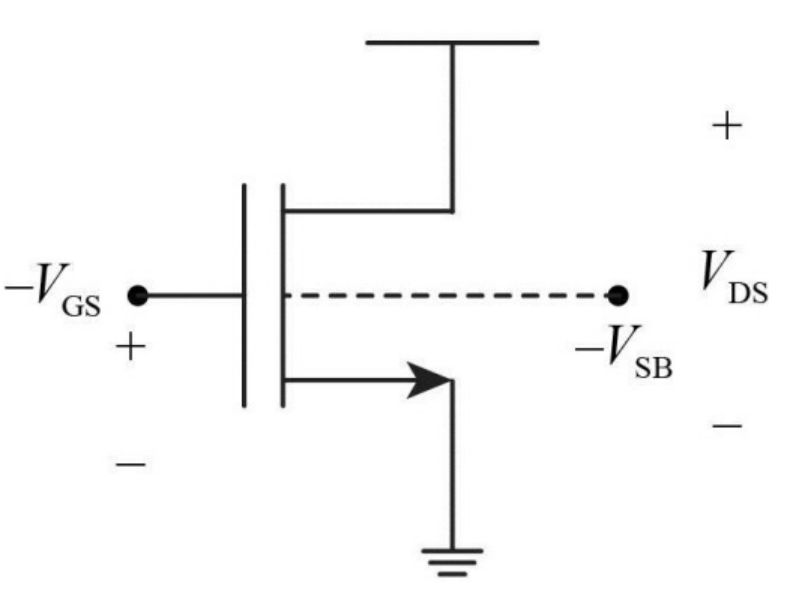
\includegraphics{2.4-1}
	\end{minipage}
	\caption*{图1:NFET的示意图} %最终文档中希望显示的图片标题
\end{figure}

(1)当$V_{GS}<V_{TH}$时,NFET关,漏电流约为零,$I_D\cong0A$

(2)当$V_{TH}<V_{GS}<V_{TH}+V_{DS}$时,NFET在饱和区,$I_D=\frac{1}{2}\mu_nC_{ox}\frac{W}{L}(V_{GS}-V_{TH})^2$

(3)当$V_{GS}>V_{TH}+V_{DS}$时,NFET在线性区,$I_D=\mu_nC_{ox}\frac{W}{L}[(V_{GS}-V_{TH})V_{DS}-\frac{1}{2}V_{DS}^2]$

(a)

	\begin{figure}[H] %H为当前位置,!htb为忽略美学标准,htbp为浮动图形
	\centering %图片居中
	\begin{minipage}{\linewidth}
		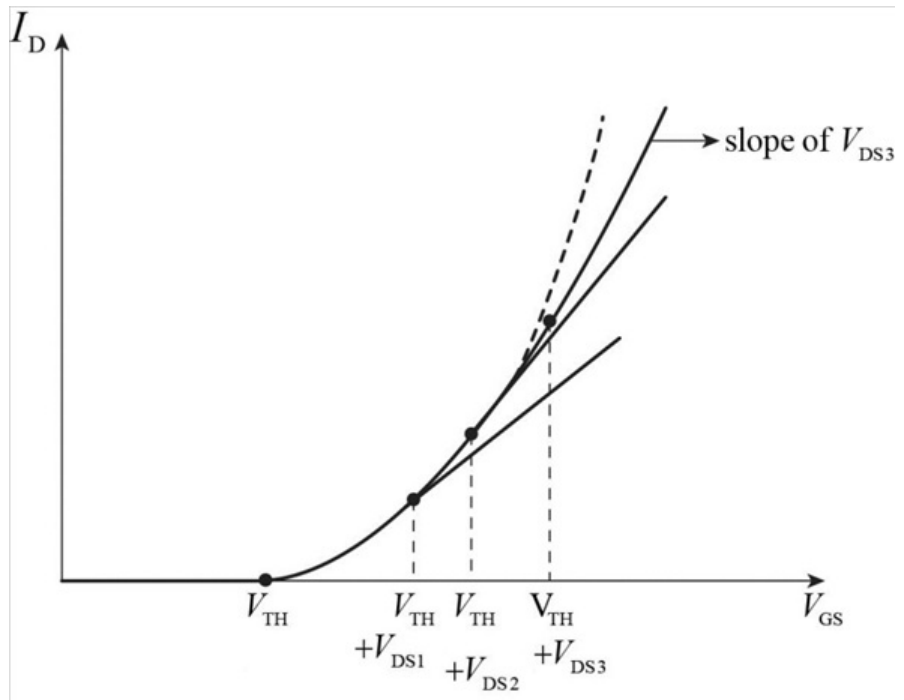
\includegraphics{2.4-2}
	\end{minipage}
	\caption*{图2:以$V_{DS}$为参数的$I_D \thicksim V_{GS}$曲线} %最终文档中希望显示的图片标题
\end{figure}

(b)

$V_{TH}=V_{TH0}+\gamma(\sqrt{|2\Phi_F+V_{SB}|}-\sqrt{|2\Phi_F|})$\textcolor{blue}{(教材P20-2.23)}

\begin{figure}[H] %H为当前位置,!htb为忽略美学标准,htbp为浮动图形
	\centering %图片居中
	\begin{minipage}{\linewidth}
		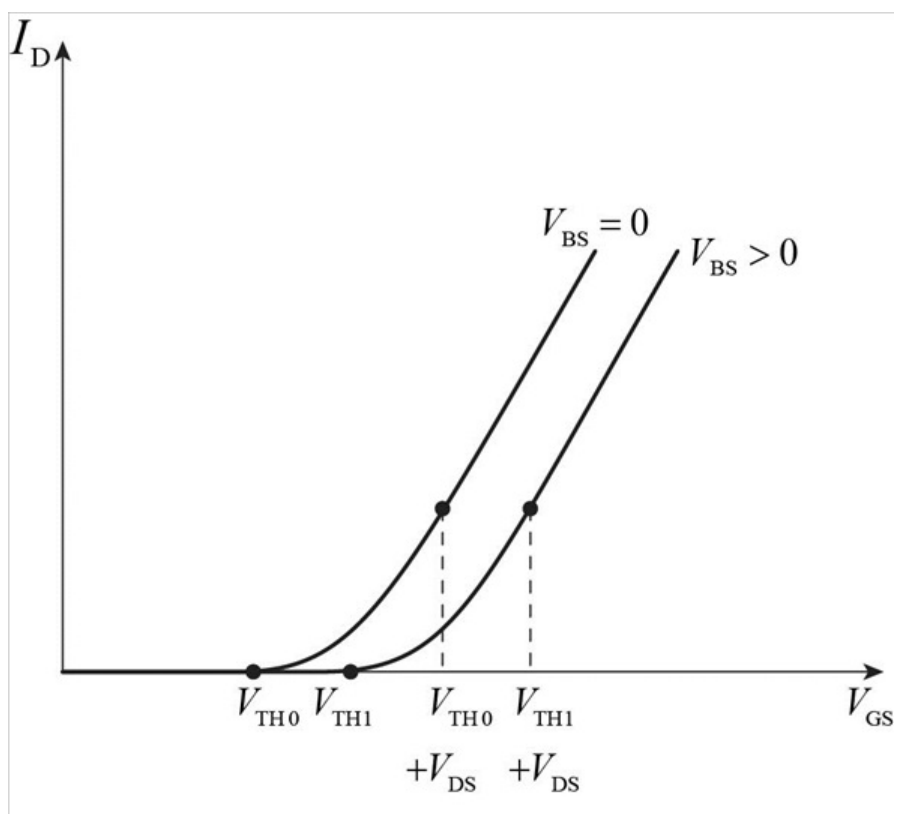
\includegraphics{2.4-3}
	\end{minipage}
	\caption*{图3:以$V_{BS}$为参数的$I_D \thicksim V_{GS}$曲线} %最终文档中希望显示的图片标题
\end{figure}